
\pagestyle{fancy} \frenchspacing
\lhead{StageControl - automatisierte Steuerung von Ton- und Lichtanlagen (2024/2025)}
\renewcommand{\chaptermark}[1]{\markboth{#1}{}}

\renewcommand{\textfraction}{0}
\renewcommand{\floatpagefraction}{0.999}
\renewcommand{\topfraction}{0.7}
\renewcommand{\bottomfraction}{0.999}
\lfoot{}

\chapter{Grundlagen und Methoden}

\section{Etablierte Lösungsansätze}
Das Kapitel listet etablierte Lösungsansätze zur Standortermittlung einer Person auf einer Bühne und erklärt diese genauer. Ebenso wie Vor- und Nachteile anhand eines Beispieles.

\subsection{Ausgangsituation des Praxisbeispiels}

Man befindet sich auf der Bühne in der Stadthalle in Ybbs. Folgende Informationen sind wichtig.
\begin{itemize}
	\item \textbf{Gerät zur Standortermittlung: } Android Smartphone
	\item \textbf{Koordinaten der Position: } TBD  
\end{itemize}

\subsection{Manuelle Steuerung}
Eine Person steht auf der Bühne der XY. Eine Möglichkeit die Steuerung der Ton- und Lichtanlagen ist diese für das Event vorher zu programmieren oder manuell während der Show zu steuern. Nun fragt sich die Person: "Wie kann ich diese Ton- und Lichtanlagen steuern?" Die Antworten folgen:

\begin{itemize}
	\item "Manuelle Steuerung der Tonanlage"
	\item "Vorprogrammierung der Lichtanlage"
\end{itemize}

An den erlangten Antworten, kann man erkennen, dass es noch keine automatisierte Lösung für das Problem gibt. Die Genauigkeit der Standortermittlung, die für die automatisierte Steuerung der Anlagen notwendig ist, kann in folgende Stufen eingeteilt werden: 

\begin{itemize}
	\item \textbf{Stufe 1: }Standort auf Bühne eingeschränkt
	\item \textbf{Stufe 2: }Standort auf Länge und Breite der Bühne eingeschränkt
	\item \textbf{Stufe 3: }Standort auf bestimmten Punkt auf der Bühne eingeschränkt
\end{itemize}

\section{Navigation}

Um die Licht- und Audioanlagentechnik richtig zu koordinieren benötigt man eine Art von Navigation. Da es sich meist um Bühnen im Innenbereich handelt, kann man keine übliche Technologie verwenden.


\subsection{GPS}
GPS (\emph{=engl. Global Positioning System}) \textcite{GPS} wird für die Standortermittlung im Außenbereich verwendet und ist für unseren Fall nicht verwendbar. Für die genaue Bestimmung von Positionen werden Satelliten verwendet.

\textbf{Funktionsweise des GPS}

Es gibt GPS-Satelliten die, die Erde zweimal pro Tag umkreisen in einer genauen Umlaufbahn. Diese Satelliten senden eindeutige Signale und Bahnparameter aus, somit können die genauen Postionen der GPS-Geräte bestimmt werden. 
In so gut wie jeden neuen Geräten ist das GPS-standart und werden für die verschiedensten Funktionen verwendet. Durch die Positionsermittlung können folgende andere Informationen berechnet werden:

\begin{itemize}
	\item Geschwindigkeit
	\item Peilung
	\item Track
	\item Reisedistanz
	\item Distanz zum Ziel
	\item Zeiten von Sonnenaufgang und Sonnenuntergang
\end{itemize}

\textbf{Signal}

Wenn GPS-Signale die Erde erreichen, sind die gesendeten Signale sehr schwach. Deshalb kommt es auch zu Problemen beim Durchdringen von Objekten wie Gebäuden o. Ä. Bei modernen GPS-Empfängern ist eine Indoor-Ortung möglich.

\textbf{Fehlerquellen für die Genauigkeit der GPS-Signale}

Es gibt einige relevante Fehlerquellen für GPS-Signale darunter fallen \textcite{GPSFehlerquellen}:
\begin{itemize}
	\item Position der Satelliten
	\item Signaleffekt der Umgebung
\end{itemize}


\textbf{Position der Satelliten}

Um ein Objekt zu positionieren sind mindestens drei Satelliten notwendig und einen weiteren, um etwägige Fehler zu beseitigen. Grundsätzlich gilt: Desto mehr Satelliten, desto genauer die GPS-Genauigkeit. Außerdem sollte das Signal von gleichmäßig verteilten Satelliten kommen, ist die GPS-Genauigkeit höher. Für die Berechnung dieser Genauigkeit gibt es den Dilution of Precision (= DOP) Wert.  Je kleiner dieser Wert, desto genauer ist das GPS-Signal.
\begin{figure}[H]
	\centering
	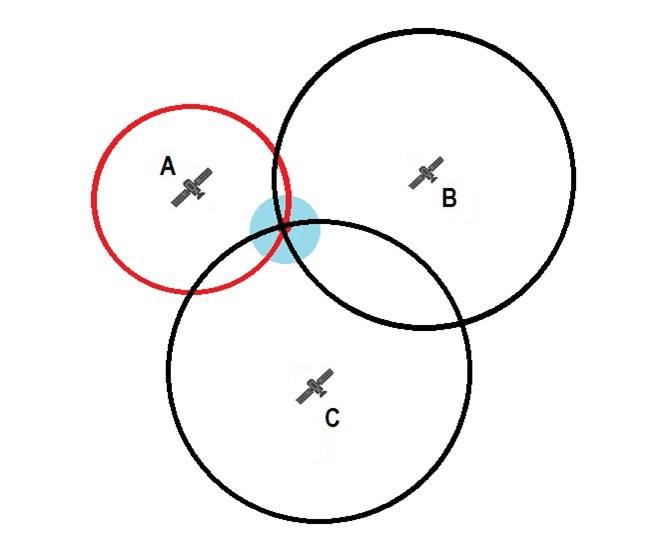
\includegraphics[width=0.7\linewidth]{images/Satellitenposition.jpg}
	\caption[Satellitenpositionierung]{Satellitenpositionierung}
	\label{fig:Satellitenposition}
\end{figure}

\textbf{Signaleffekt der Umgebung}

Bis die Signale von Satelliten schlussendlich beim GPS-Empfänger ankommen legen sie eine lange Stecke zurück, die Ausbreitungsumgebung beinflusst nicht nur die Siganlestärke, sondern auch die Genauigkeit, stark.
\begin{figure}[H]
	\centering
	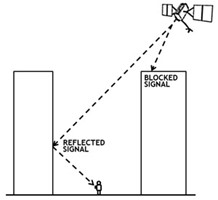
\includegraphics[width=0.7\linewidth]{images/Satelliteneinfluss.jpg}
	\caption[Satelliteneinfluss]{Satelliteneinfluss}
	\label{fig:Satelliteneinfluss}
\end{figure}


\subsection{ESP32}

ESP32 ist eine Reihe von Chip-Mikrocontrollern, die von dem Unternehmen Espressif entwickelt wurden und mit Hilfe von Arduino bzw. der Programmiersprache C kommunizieren. Der ESP32 \textcite{ESP32} zeichnet sich mit folgenden Dingen aus:

\begin{itemize}
	\item niedrige Anschaffungskosten
	\item geringer Stromverbrauch
	\item Wi-Fi
	\item Bluetooth
\end{itemize}


\begin{figure}[H]
	\centering
	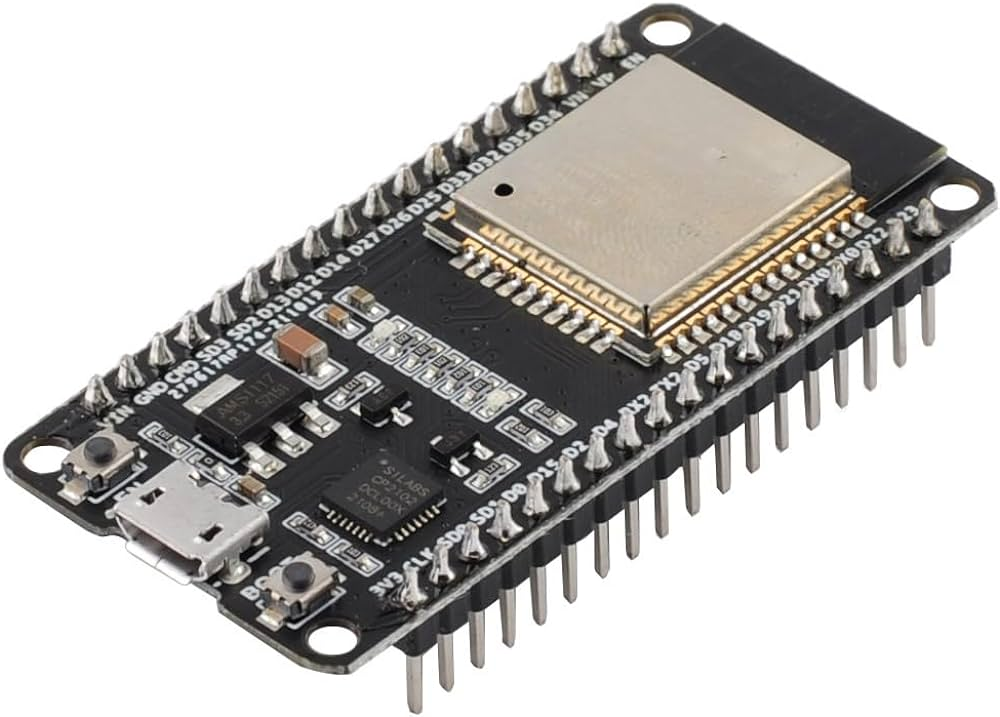
\includegraphics[width=0.7\linewidth]{images/ESP32.jpg}
	\caption[ESP32]{ESP32}
	\label{fig:ESP32}
\end{figure}

\textbf{Anschaffungskosten \& Stromverbrauch}

Der Mikrocontroller ist bereits ab einem Preis von \$6 erhältlich. Außerdem verbraucht dieser im Vergleich zu anderen Mikrocontrollern sehr wenig Strom und unterstützt Energiesparmodule, wie Tiefschlaf.

\textbf{Funktionen}

Der Mikrocontroller bietet nicht nur Wi-Fi (\emph{=Wireless Local Area Network}), sondern auch Bluetooth. Mit der Wireless Local Area Network Funktionen kann man einfach und drahtlos eine Verbindung zu einem Netzwerk herstellen und somit eine Kommunikation von vielen Geräten möglich machen. Außerdem verfügt der Mikrocontroller über Bluetooth-Classic.

\subsection{ESP32-Spezifikationen}

\begin{itemize}
	\item Bluetooth Classic und Bluetooth Low Energy
	\item Tensilica Xtensa Dual-Core 32-Bit LX6 Mikroprozessor, 160 oder 240 MHz
	\item ROM:  448 KB
	\item SRAM:  520 KB 
\end{itemize}

\subsection{MPU-6050}

Für weitere Funktionen benötigt man z.B. die Erweiterungsplatine MPU-6050, diese bringt einen Beschleunigungssensor und ein Gyroskop mit. Diese Platine beläuft sich auf einen Preis von ca. \$3.

\begin{figure}[H]
	\centering
	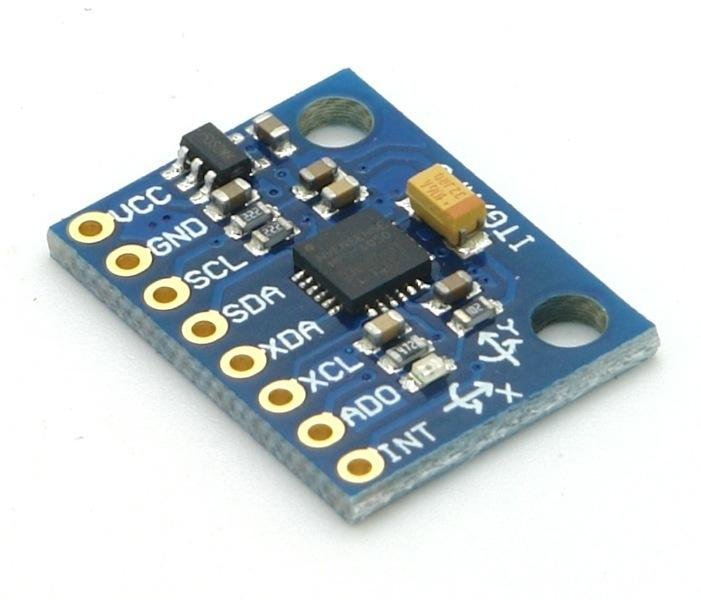
\includegraphics[width=0.7\linewidth]{images/MPU6050.jpg}
	\caption[MPU6050]{MPU-6050}
	\label{fig:MPU6050}
\end{figure}


\textbf{Gyroskop}

Jeder kennt die Wirkung eines Kreisel, ein Gyroskop hat genau diese und wird deshalb auch Kreiselinstrument genannt. Man nutzt die Wirkung, um die Lage eines Objektes zu bestimmen. Im Falle von einem MPU-6050 wird ein Sensor namens Micro-Electric-Mechanical Systems (\emph{kurz MEMS}) verwendet. 


\begin{figure}[H]
	\centering
	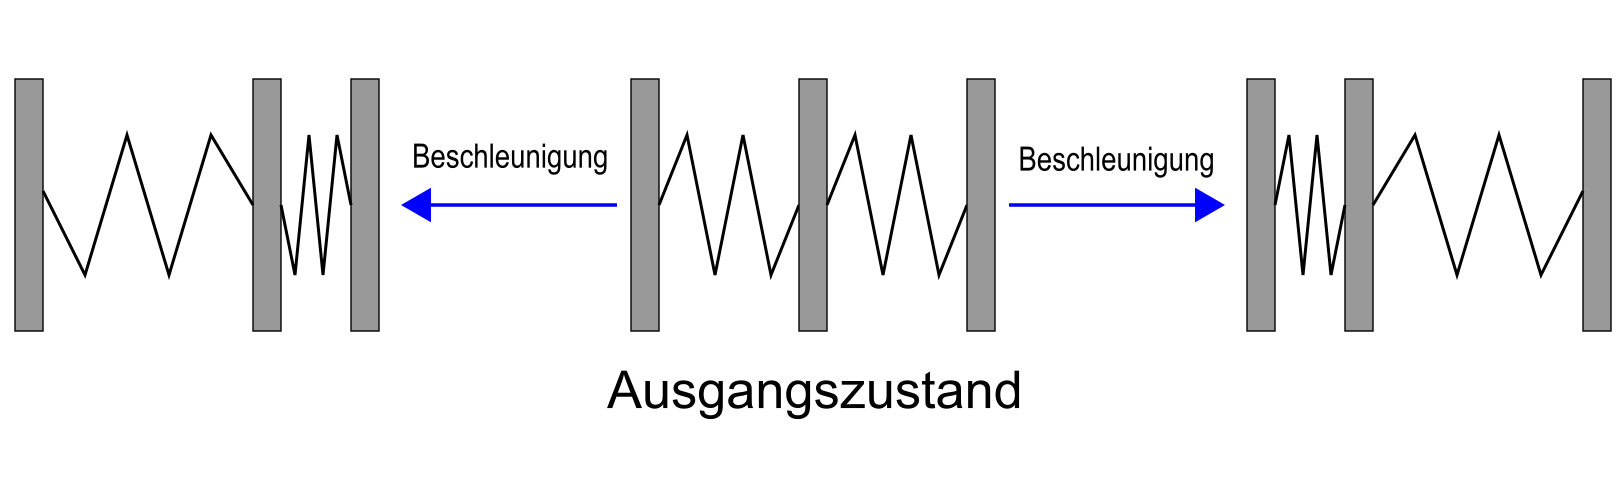
\includegraphics[width=0.7\linewidth]{images/Beschleunigungssensor.png}
	\caption[Beschleunigungssensor]{Beschleunigungssensor}
	\label{fig:Beschleunigungssensor}
\end{figure}

\textbf{Beschleunigungssensor}

Ein Beschleunigungssensor funktioniert nach dem selben Prinzip, wie ein Gyroskop. Der einzige Unterschied ist, dass der Sensor die Beschleunigung in Richtung der x-, y- und z-Achse deklariert. Ein Gyroskop bezieht sich lediglich auf die Bewegung, um die Achsen, also befindet es sich in Ruhestellung, liefert es den Wert Null für alle drei Dimensionen (x,y,z). \textcite{MPU6050} Die Module haben die Achsen aufgedruckt.

\begin{figure}[H]
	\centering
	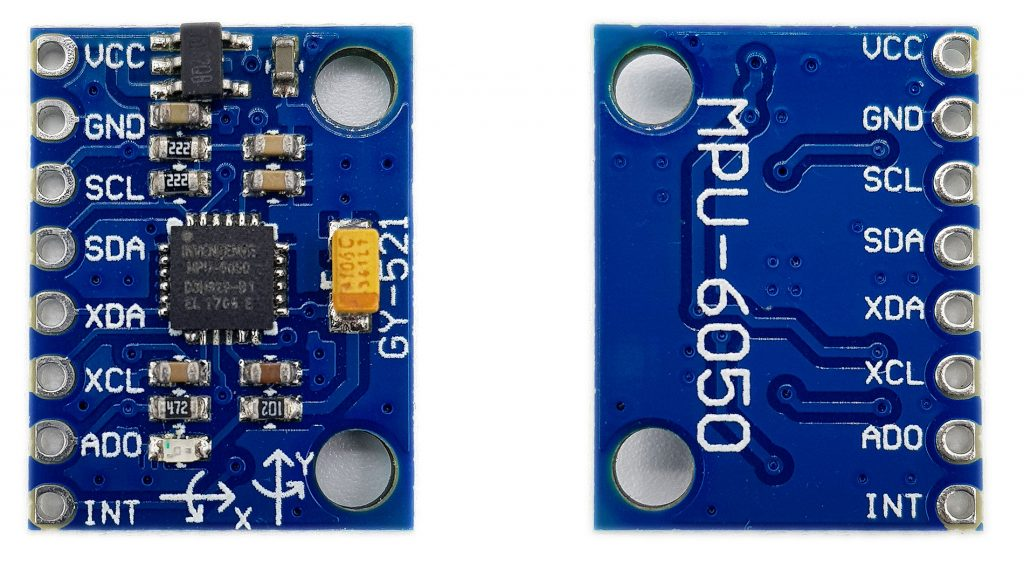
\includegraphics[width=0.7\linewidth]{images/Modul.jpg}
	\caption[Modul]{Modul}
	\label{fig:Modul}
\end{figure}

\subsection{Trägheitsnavigation}

Die Trägheitsnavigation nutzt die physikalische Eigenschaften der Trägheit, um fortlaufende Berechnung der Position, Orientierung und Geschwindigkeit eines Objekts zu ermöglichen. \textcite{Traegheitsnavigation} Es ist immer nur die Anfangsposition bekannt, anhand dieser wird die spätere Position eines Objektes errechnet. Auch in GPS-gestörten Umgebungen z.B. Gebäuden, funktioniert die Trägheitsnavigation. 


\section{Software}


\subsection{Mobil Apps Grundlagen}

\textbf{Native Apps}

Native Apps (\emph{=deu.: angepasste Anwendung}) sind Anwendungen, die speziell für ein Betriebssystem (Android, iOS) entwickelt wurden. \textcite{NativeApps}

\textbf{Android}

Android ist einer der weltweit Bekanntesten Betriebssysteme, es ist akutell auf 2,5 Milliarden aktiven Geräten installiert. \textcite{Android} Weiters ist Android ein Open-Source Betriebssystem, es ist offen für Entwickler.  

\textbf{iOS}

Das Betriebssystem iOS wurde von Apple im Jahre 2007 veröffentlicht. \textcite{iOS} Die Software wird bei iPhone und iPad verwendet. Anders wie bei Android ist iOS nicht quelloffen, außerdem werden keine Betriebssystem-Lizenzen vergeben. Man benötigt eine gültige Apple-ID, um das Gerät zu verwenden.

\subsection{Cross-Platform-Apps}

\textbf{Flutter}

Flutter ist eine Open-Source-Software, welche von Google entwickelt worden ist.\textcite{Flutter} Der Vorteil dieses Frameworks ist, dass man mit einem Programmcode in Flutter mehreren Apps auf verschiedenen Plattformen (Android, iOS) erstellen kann. Die Hauptprogrammiersprache ist Dart.

\textbf{React Native}

React Native ist eine Open-Source-Software, welche von Facebook entwickelt worden ist. \textcite{ReactNative} Es wurde entwickelt, um Entwicklern mit Erfahrungen in React die Möglichkeit zu geben, einfacher Android Apps basierend auf React zu entwicklen. Die Hauptprogrammiersprachen sind JavaScript oder TypeScript.

\subsection{App-Entwicklung}

Für die App-Entwicklung wird Android Studio verwendet. 

Um Android Studio verwenden zu können muss man eine SDK (\emph{=engl. Software Development Kit}) installieren. \textcite{AppEntwicklung} Außerdem ist IntelliJ IDEA Community/Ultimate als IDE (\emph{=engl. Integrated Development Environment}) vorgesehen. Diese enthält die wichtigsten Programmierwerkzeuge und Programmierbiblotheken. Der Entwickler, selbst, entscheidet darüber, welche Programmiersprache verwendet wird. Es besteht die Auswahl zwischen Java, Kotlin, Ruby oder sogar C++.


\textbf{IntelliJ IDEA}

IntelliJ IDEA ist einer der beliebtesten IDEs für Java und Kotlin, die es auf den Markt gibt. Das Unternehmen, welches die Software entwickelt hat, heißt JetBrains. 

Es gibt zwei verschiedene Versionen:
\begin{itemize}
	\item IntelliJ IDEA Community Edition
	\item IntelliJ IDEA Ultimate
\end{itemize}

Die beiden Versionen unterscheiden sich minimal, denn die Ultimate Version bietet z.B. JavaScript Integration oder "duplicate detection". \textcite{IntelliJ}

\begin{figure}[H]
	\centering
	\includegraphics[width=0.5\linewidth]{images/intelliJ.png}
	\caption[IntelliJ]{IntelliJ}
	\label{fig:IntelliJ}
\end{figure}

\textbf{Eclipse}

Eclipse ist eine weitere bekannte IDE, die Software umfasst 48\% des Marktanteils. Man kann nicht nur in Java programmieren, sondern mit den entsprechenden Plugins auch in Python, JavaScript oder C++. Außerdem läuft es auf jeder Platform, Linux, macOS oder Windows, \textcite{Eclipse}.

\begin{figure}[H]
	\centering
	
\includegraphics[width=0.5\linewidth]{images/eclipse.png}
	\caption[Eclipse]{Eclipse}
	\label{fig:Eclipse}
\end{figure}







\begin{figure}[H]
	\centering
	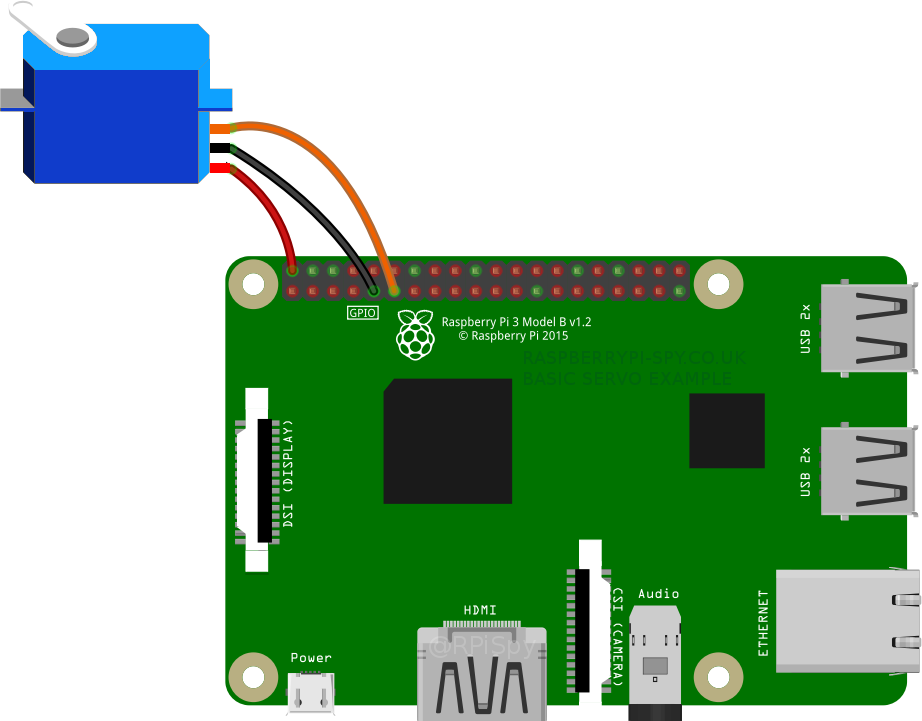
\includegraphics[width=0.7\linewidth]{images/Pin_Belegung.png}
	\caption[Pin-Belegung Servo]{Pin-Belegung Servo}
	\label{fig:PIN_Belegung}
\end{figure}






\chapter{Ergebnisdokumentation}
\textbf{TBD}


